\documentclass[12pt]{article}
\usepackage{natbib}
\usepackage{hyperref}
\usepackage{graphicx}
\usepackage{subcaption}
\usepackage{amssymb,amsmath,amsthm}
\usepackage{xcolor}
\usepackage{xspace}
\usepackage[nameinlink,capitalize]{cleveref}
\usepackage{cleveref}
\usepackage[margin=1in]{geometry}
\usepackage{lineno}\renewcommand\thelinenumber{\color{gray}\arabic{linenumber}}
\usepackage{pdflscape}
\usepackage{array}
\usepackage{tikz}
\usepackage{authblk}

\newcolumntype{L}[1]{>{\raggedright\let\newline\\\arraybackslash\hspace{0pt}}m{#1}}
\newcolumntype{C}[1]{>{\centering\let\newline\\\arraybackslash\hspace{0pt}}m{#1}}
\newcolumntype{R}[1]{>{\raggedleft\let\newline\\\arraybackslash\hspace{0pt}}m{#1}}

\newcommand{\comment}{\showcomment}
\newcommand{\showcomment}[3]{\textcolor{#1}{\textbf{[#2: }\textsl{#3}\textbf{]}}}
\newcommand{\nocomment}[3]{}
\newcommand{\pkg}[1]{\textsf{#1}}  %{\texttt{#1}}
\newcommand{\ncurve}{\ensuremath{N_{\textrm{curves}}}\xspace}
\newcommand{\nsample}{\ensuremath{N_{\textrm{samples}}}\xspace}
\newcommand{\juul}{Juul \emph{et al.}\xspace}  %% ref w/o year and hyperlink

\newcommand{\ali}[1]{\comment{magenta}{Ali}{#1}}
\newcommand{\bmb}[1]{\comment{red}{BMB}{#1}}
\newcommand{\todo}[1]{\comment{red}{TODO}{#1}}

\theoremstyle{definition} % amsthm only
\newtheorem{proposition}{Proposition}
\newtheorem{theorem}{Theorem}
 
\bibliographystyle{apalike}

\title{Additional details on functional boxplots}
% \author{Ali Gharouni, Benjamin M. Bolker}
\author[1]{Ali Gharouni}
\author[1,2,3]{Benjamin M. Bolker}

\affil[1]{Department of Mathematics \& Statistics, McMaster University, Hamilton, Canada}
\affil[2]{Department of Biology, McMaster University, Hamilton, Canada}
\affil[3]{Michael G. DeGroote Institute for Infectious Disease Research, McMaster University, Hamilton, Canada}
\begin{document}
\maketitle
\linenumbers

\cite{juul2021fixed} pointed out shortcomings to the standard ways that researchers draw confidence intervals for ensembles of curves, with specific examples drawn from the output of stochastic epidemic models. In particular, they showed that fixed-time approaches (e.g., computing pointwise quantiles) can fail to capture the uncertainty in key features of an epidemic such as the timing and magnitude of epidemic peaks.  As an alternative to fixed-time approaches, the authors illustrated methods to compute the \emph{central set} of an ensemble of curves, a high-dimensional analogue of interquartile range or confidence interval. There is a large body of literature on this topic under the rubrics of \emph{functional depth} and \emph{functional boxplots} for high dimensional data \citep{fraiman2001trimmed, lopez2007depth, lopez2009concept, sun2011functional,sun2012exact}. While \juul do cite this literature \citep{sun2011functional}, exploring it in more depth led us to several useful practical and theoretical points that could be useful for researchers interested in using these approaches.

\juul's primary method for determining a curve's centrality (and hence whether it should be included in a central set of curves for display) was to measure the fraction of times that a given curve is completely included within the envelope of a set of other curves randomly sampled from the ensemble. \juul chose the number of curves [or \emph{tuning parameter}] as $J=50$ (they use the notation \ncurve), and chose $\nsample=100$ such samples to compute the fraction (\emph{band depth}) for each curve. They provided open-source Python code that implements this method, as well as some of the weighted variants they discuss. For the simple (unweighted) case, however, there are already mature open source implementations available in R \citep{fda_pkg,roahd}, Matlab (\url{https://www.psych.mcgill.ca/misc/fda/downloads/FDAfuns/}), and Python \citep{seabold2010statsmodels}. In general these packages use the same functional band depth measure as \juul, but substituting $J=2$, which is robust \citep{lopez2009concept} and allows the use of a computationally efficient algorithm for large data sets \citep{sun2012exact}. 
It is unclear why \juul chose larger values of $J$ (10 and 50), although the dimensions of their examples are small enough that the computational burden is not important.

\juul also suggest ranking according to a single, one-dimensional feature of interest such as the maximum values of newly hospitalized cases in a single day (their Fig.~2e). We suggest that this approach could be extended to incorporate multiple features of interest. Functional band depth could again be used on this reduced set of features; here we use the \emph{Mahalanobis distance} \citep{mahalanobis1936generalized}, which measures distance from a centroid accounting both for variation in the scales or typical magnitudes of different features and for correlation among features.
Our example uses a feature set including the peak value of incidence (new infections), the time at which the peak occurs, and the initial growth rate, duration, and final size of the epidemic. While these are typical epidemiological features of interest, researchers can and should choose the features that are most closely connected to their particular research questions \citep{probert2016decision}.

\begin{figure}[h!]
  \centering
  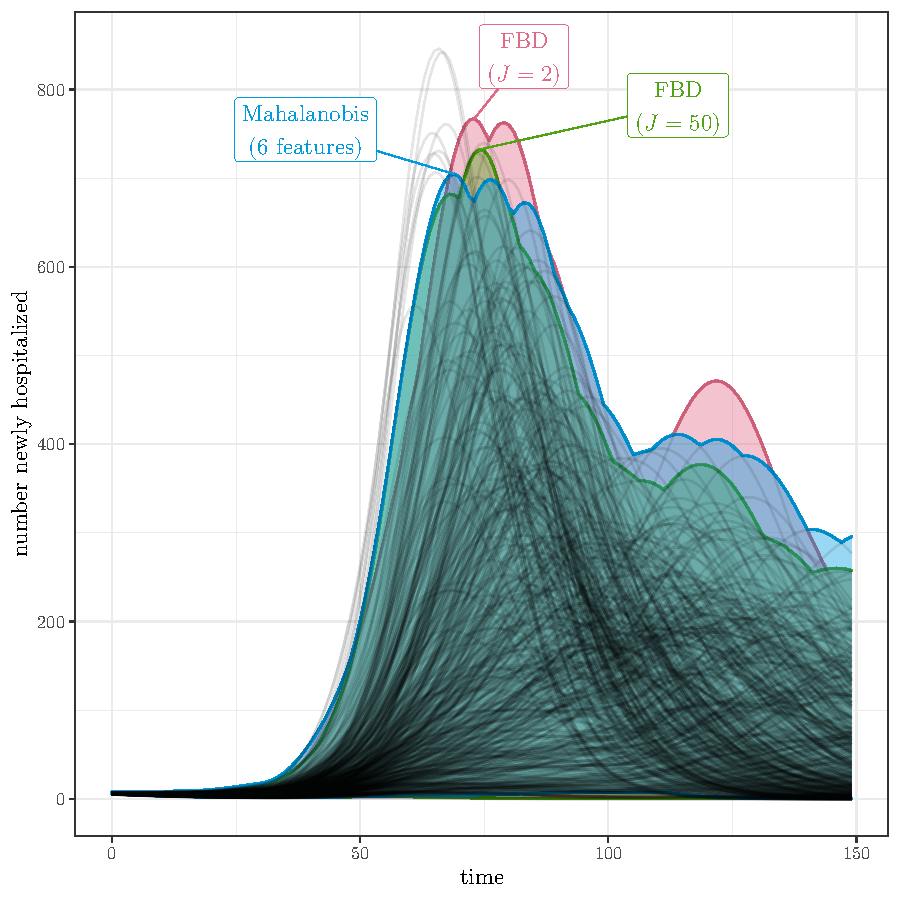
\includegraphics[width=\linewidth]{scripts/cent_plot.pdf}
  \caption{Comparison of 90\% central regions computed with
    different functional boxplot methods, using epidemic curve ensembles from \juul. FBD = functional band distance; $J$ = number of curves used for centrality calculation. Curve with $J=2$ computed via the \texttt{roahd} package \citep{roahd}: curve with $J=50$ used our own implementation of the functional band distance algorithm described by \juul.
  }
  \label{p.a}
\end{figure}
  
\bibliography{./CurveBP}
\end{document}
